\clearpage

\section{Softwaredesign}
Dette afsnit beskriver designprocessen af softwaren. Afsnittet tager udgangspunkt i UC1, som er systemets vigtigste use case nemlig at måle og vise blodtryk. Her er der arbejdet iterativt, da det var nødvendigt at udvide softwaren mange gange i forhold til det oprindelige design. For at illustrere dette viser nedenstående figur første version af et sekvensdiagram for UC1. 

\begin{figure}[h!]
	\centering
	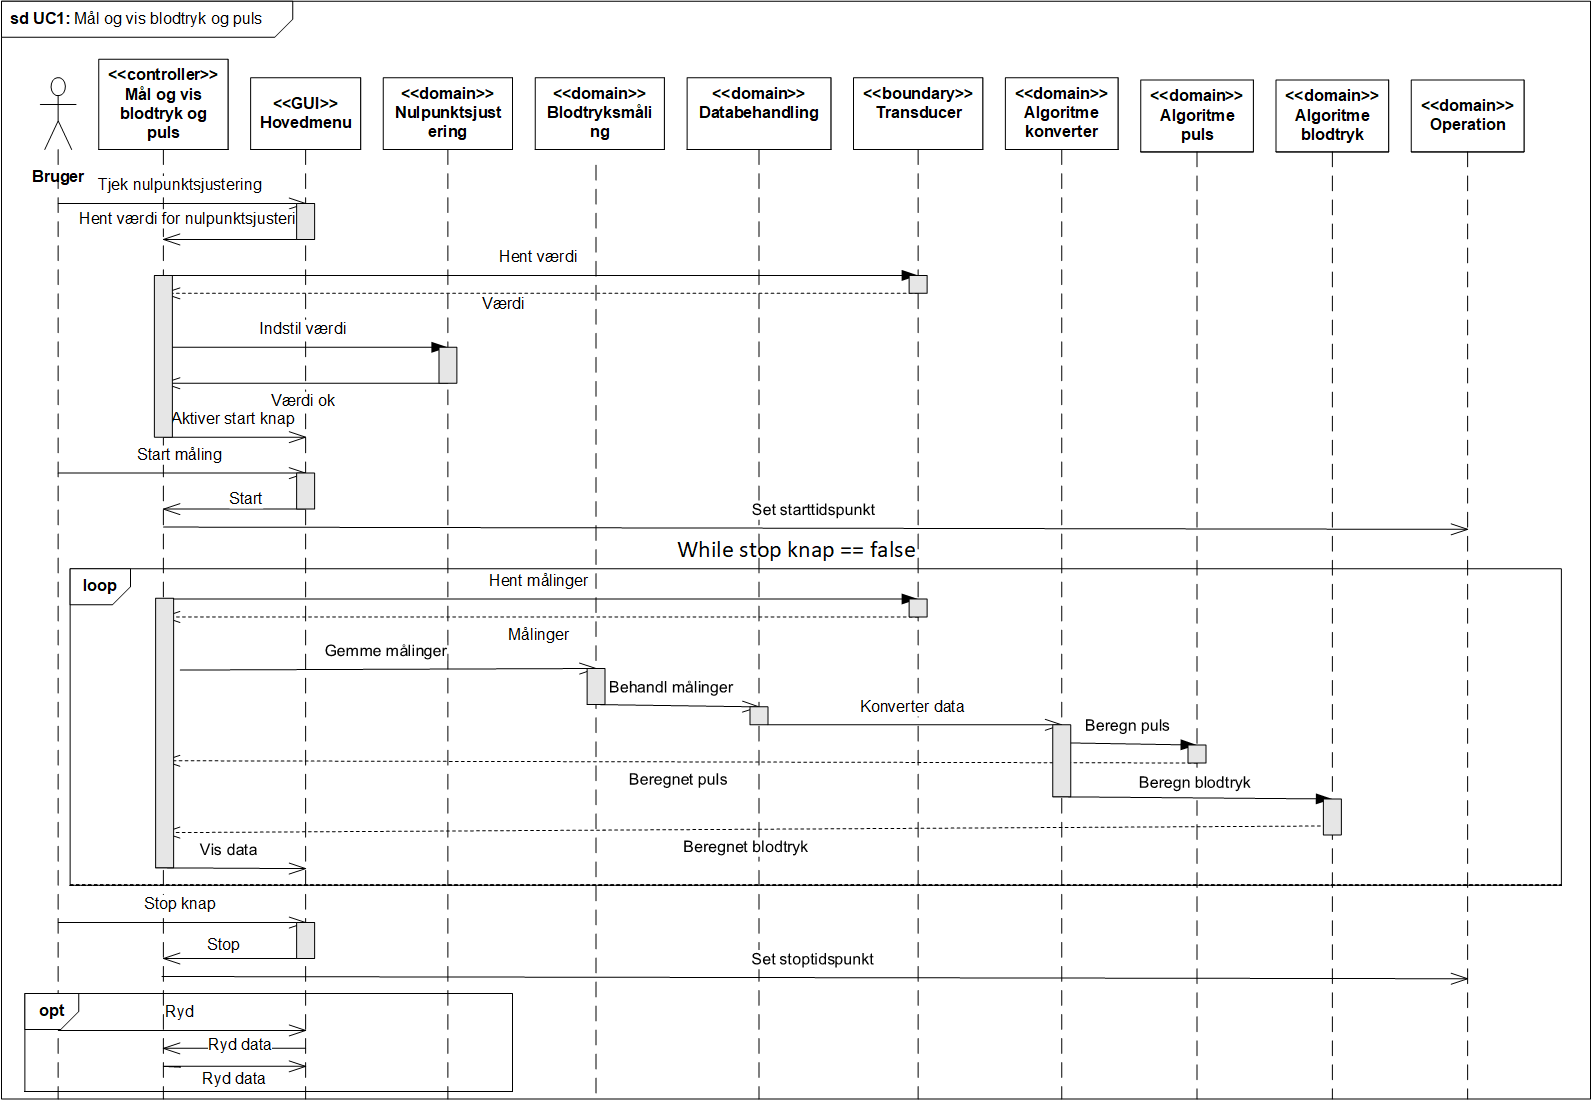
\includegraphics[width=1\linewidth]{Arkitektur_og_design/Softwarearkitektur/sekvens_uc1_version1}
	\caption{Sekvensdiagram for Use Case 1 (første version)}
	\label{fig:sekvensdiagram_ver1}	
\end{figure}

Som det ses ud fra diagrammet, var der på dette tidspunkt ikke indbygget en producer-consumer struktur med en datacontainer i designet. Desuden var der også en domæneklasse kaldet Databehandling, som det senere viste sig ikke var nødvendig. Det overordnede princip er dog stadig det samme som den endelige implementering af UC1, som kan ses i \ref{fig:sekvensdiagram_ver2}. Dette viser at iterationerne af UC1 har været mange små forbedringer fremfor et komplet redesign af use casen. Nedenstående figur viser det endelige sekvensdiagram for UC1. For større visning af figuren henvises til bilaget. 

\clearpage
\vspace{0.5 cm}
\begin{figure}[h!]
	\centering
	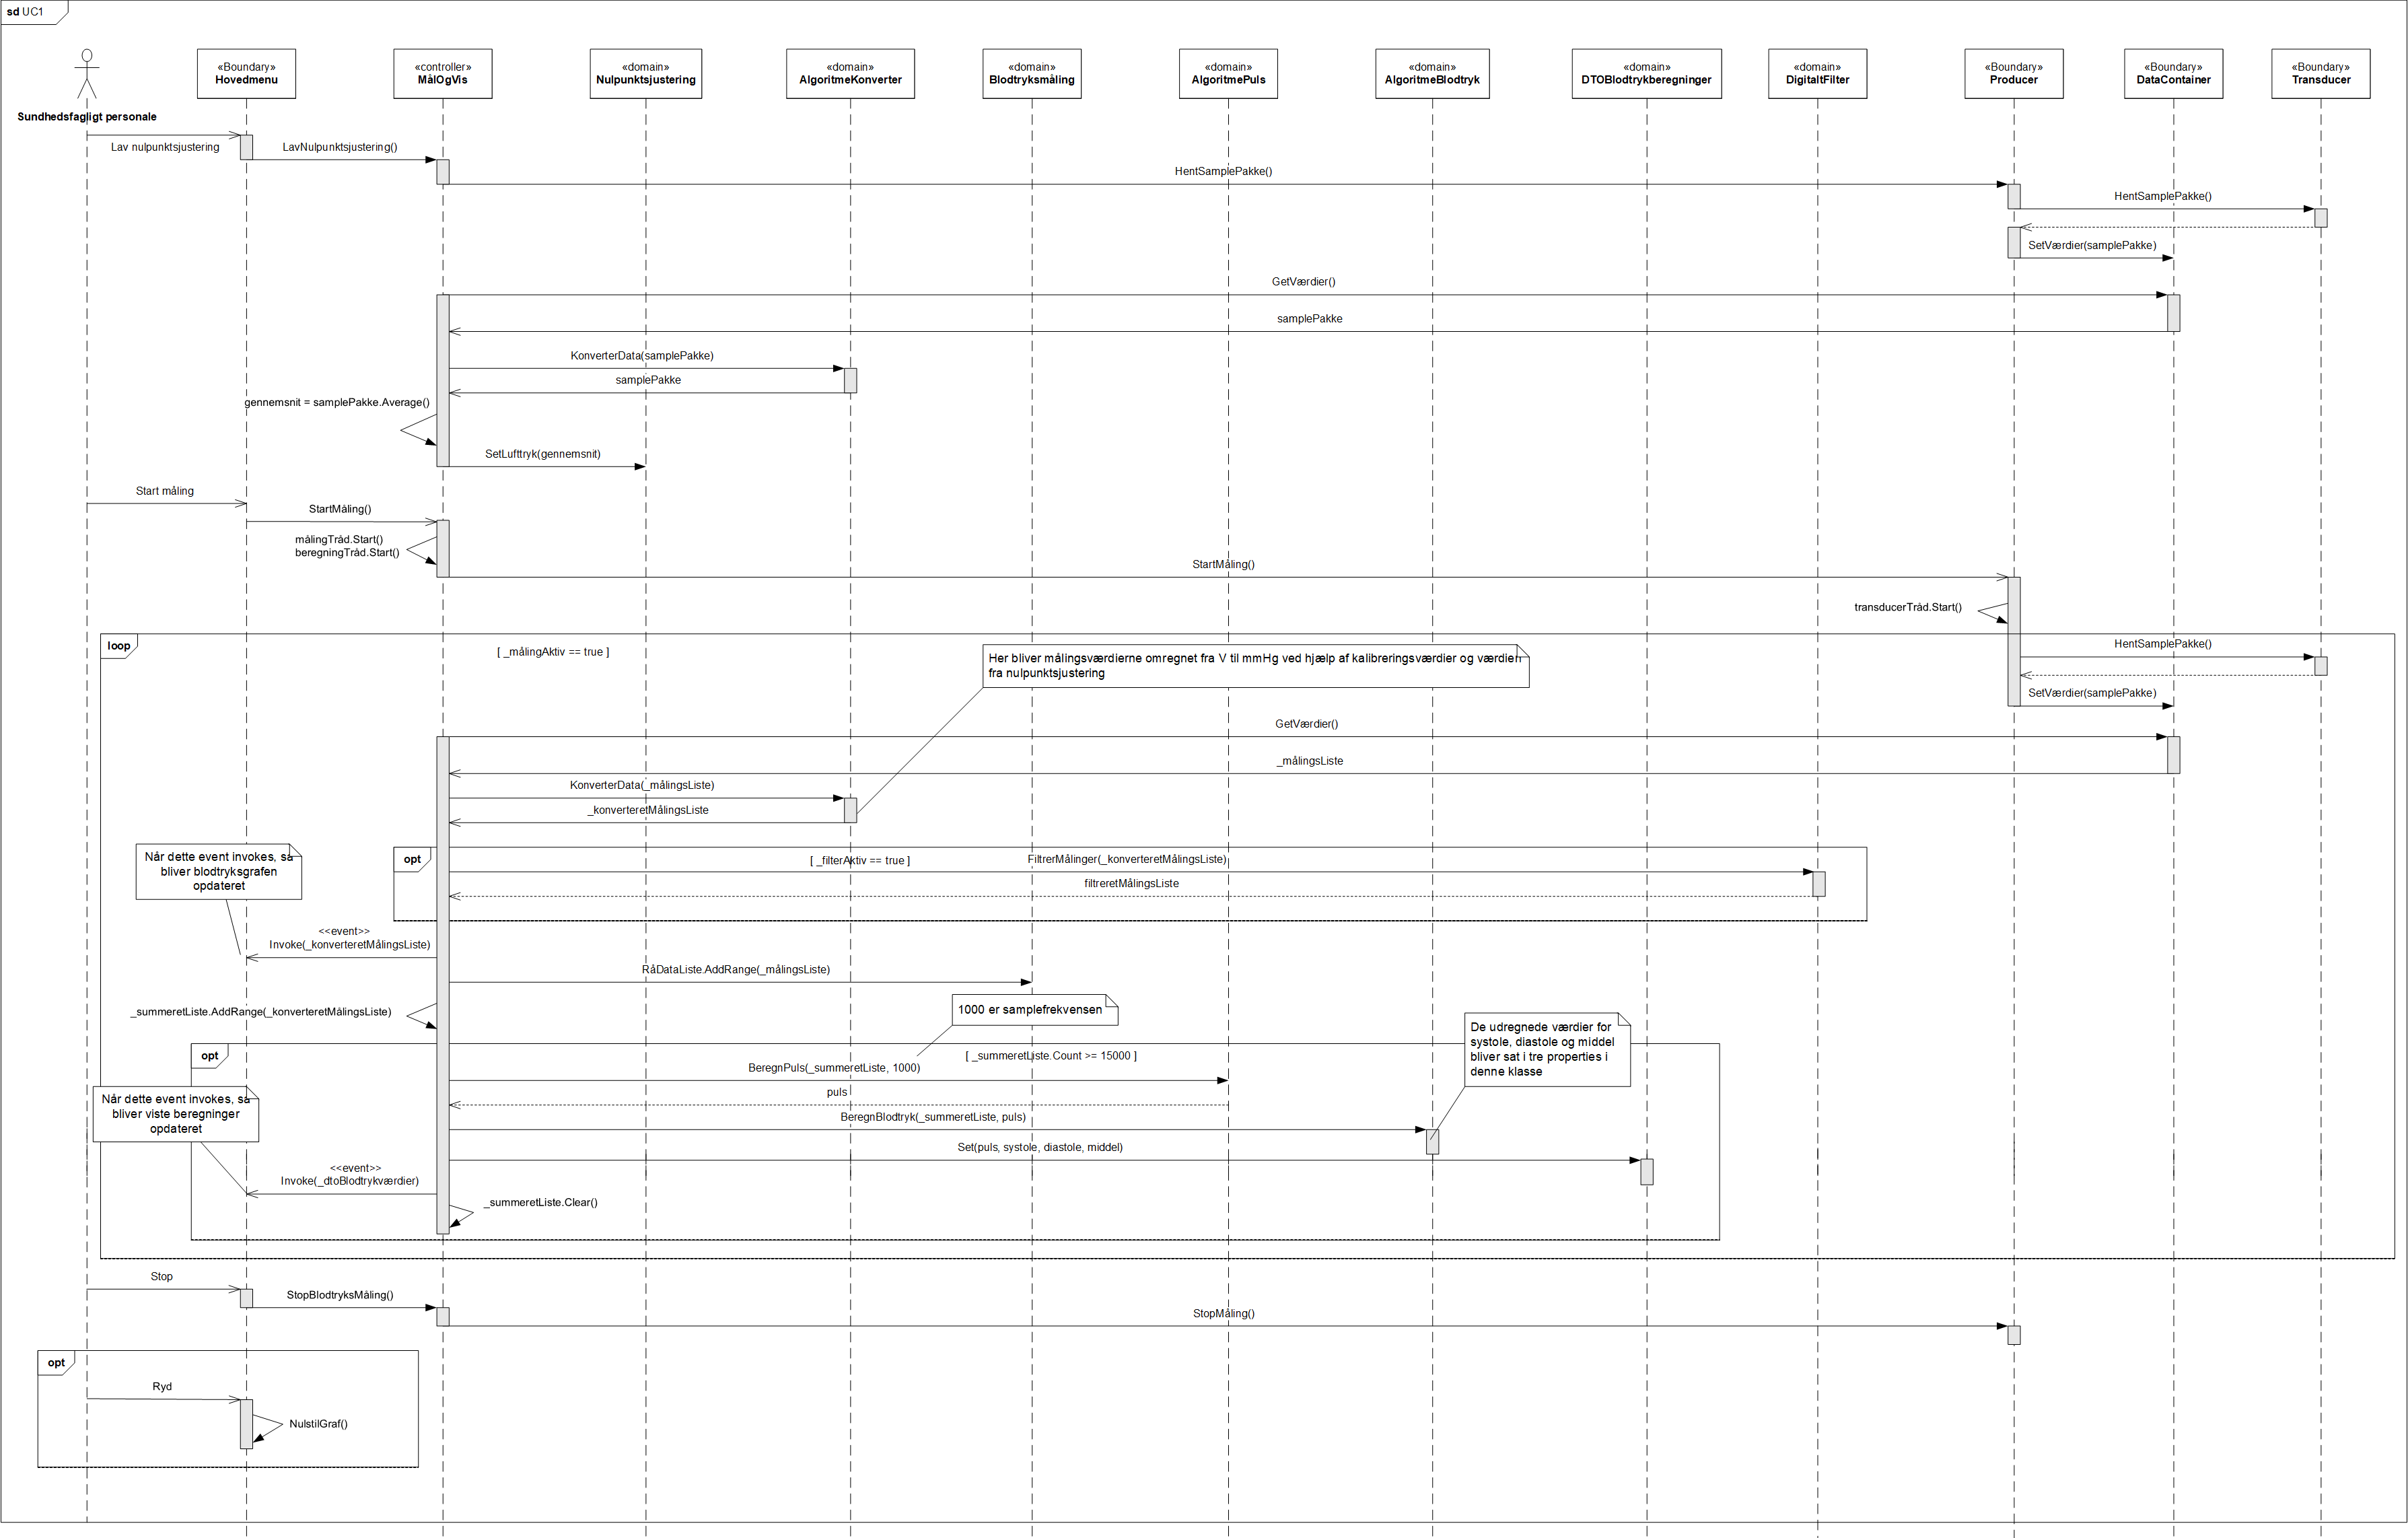
\includegraphics[width=1\linewidth]{Arkitektur_og_design/Softwarearkitektur/sekvensdiagram}
	\caption{Sekvensdiagram for Use Case 1: Mål og vis blodtryk og puls (endelig version)}
	\label{fig:sekvensdiagram_ver2}	
\end{figure}
\vspace{0.5 cm}

Sekvensdiagrammet viser interaktionen mellem de forskellige klasser, og hvilke oplysninger der bliver sendt rundt. Den første del af diagrammet beskriver nulpunktsjusteringen, som sker inden en måling kan igangsættes. Den midterste del som er indrammet af et loop beskriver selve målingen og opdateringen af GUI’en.  Der er benyttet tråde, hvilket ikke direkte kan illustreres på et sekvensdiagram. Som det er vist ovenstående, sker opdateringen af grafen inden opdateringen af beregningerne. I virkeligheden forløber opdatering af grafen, og opdatering af beregninger sideløbende i to tråde. Dette kunne være vist i et aktivitetsdiagram, men dette er ikke udarbejdet, da andet har været prioriteret højere. 

Måling og beregninger sker indtil sundhedsfagligt personale vælger at stoppe målingen. Dette er vist nederst i diagrammet. Ud fra sekvensdiagrammet er der udarbejdet et udfyldt klassediagram, som beskriver alle attributter og metoder der er nødvendige for at realisere Use Case 1. For større visning af figuren henvises til bilaget.

\clearpage
\begin{figure}[h!]
	\centering
	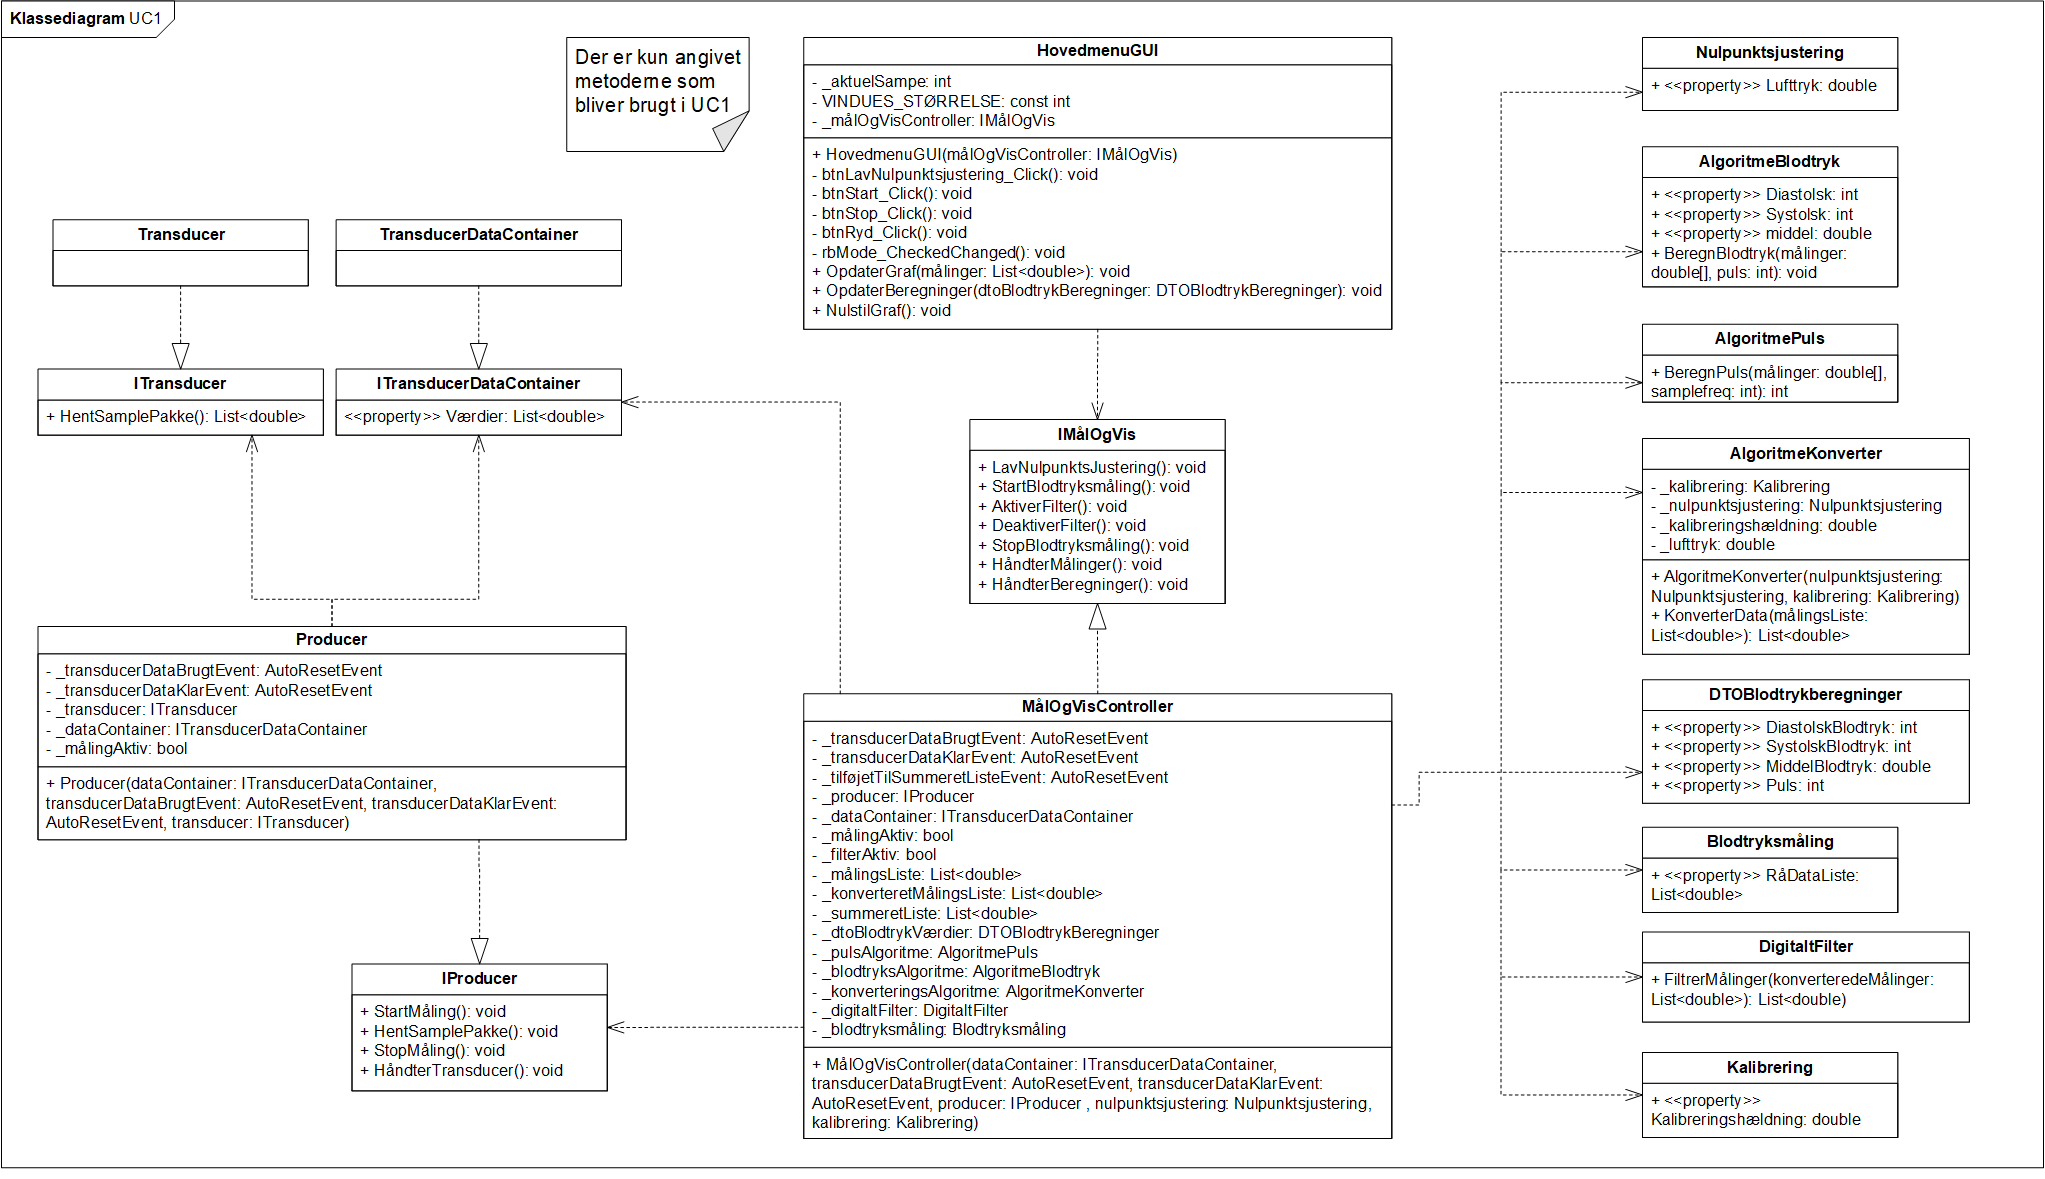
\includegraphics[width=1\linewidth]{Arkitektur_og_design/Softwarearkitektur/classdiagram}	
	\caption{Klassediagram udfyldt med attributter og metoder}
	\label{fig:classdiagram}
\end{figure}
\vspace{0.5 cm}

Som der står på diagramnoten, så er der kun inkluderet metoder og attributter, som bruges i UC1. Diagrammet er forsøgt delt op i tre kolonner. Alle klasserne der ses til højre er domæneklasser, som en del af domæne package jf. \vref{fig:tomclass}. I midterste kolonne er der HovedmenuGUI klassen, som er en del af PL, samt interfacet IMålOgVis og MålOgVisController, som er en del af BL. Det er underforstået, at klasser der implementerer et interface indeholder interfacets metoder. Klasserne til venstre i diagrammet er en del af DAL. Ud fra klassediagrammet er det tydeligt, at UC1 er forholdvis kompleks og indeholder rigtig mange afhængigheder. Dette gav sig til udtryk ift. test, da det viste sig at være meget sværere at lave unittests på denne use case end forventet. Dette er nærmere beskrevet i testafsnittet.

\clearpage
\vspace{1 cm}
\textbf{Puls}

\begin{figure}[h!]
	\centering
	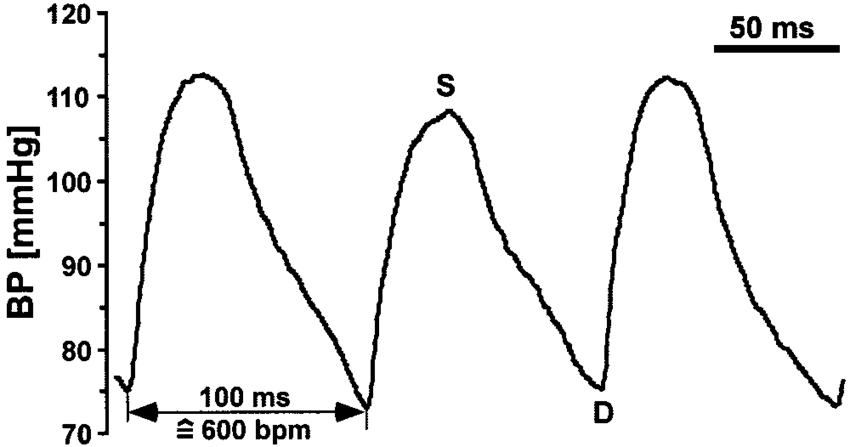
\includegraphics[width=0.5\linewidth]{Arkitektur_og_design/Softwarearkitektur/puls}	
	\caption{Puls}
	\label{fig:puls}
\end{figure}

Et af vores must have krav er, at vi skal kunne vise systolis-, diastolisk-, middelblodtryk og puls på brugergrænsefladen. Derfor skal vores system kunne finde pulsen ud fra et blodtrykssignal. Dette kunne løses på to måder. Den ene mulighed var at måle tiden mellem to diastoler, da hjertet på denne tid har kontraheret sig og pumpet blod ud i det store kredsløb. Dette kan ses på figur \vref{fig:puls}. Denne metode vil dog kun give en indikation om, hvad pulsen er, men vil ikke kunne give den nøjagtige.
Den anden mulighed var at lave fourier transformation på blodtrykssignalet. Ved at lave fourier transformation vil vi flytte blodtrykssignalet fra tidsdomænet til frekvensdomænet. På frekvensspekteret vil vi kunne finde den måling med den højeste amplitude. Den måling med den højeste amplitude er den måling med mest energi i, og dermed den frekvens, der optræder flest gang i signalet. Denne måling har en frekvens, og ved at gange denne med 60, vil vi få vores puls. Vi har valgt at arbejde med denne metode i det, man beregner pulsen over en længere periode, og dermed vil det give en mere præcis indikation på pulsen.

Den beregnede puls benytter vi til at beregne det systoliske-, diastoliske-, og middelblodtrykekt. Pulsen er med til at bestemme, hvor langt tilbage i blodtrykssignalet vi skal gå for at finde minimum, maximum og middelværdien. Minimum er det diastoliske, maxiumum er det systoliske og middelværdien er middelblodtrykket.

For at give et overblik til os selv om, hvordan beregninger af puls og blodtryksværdierne skulle foregå ville det have været en fordel, at vi havde lavet aktivitetsdiagrammer.
